%\documentclass[english, times, mirror]{revdetua}
% use this if you're writing in portuguese:
\documentclass[portuguese, times, mirror]{revdetua}

\usepackage[utf8]{inputenc}
\usepackage{graphicx}
\usepackage{hyperref}

\usepackage{amsmath}
\usepackage{mathtools}

\usepackage{caption}
\usepackage{listings}
\usepackage{color}

\definecolor{dkgreen}{rgb}{0,0.6,0}
\definecolor{gray}{rgb}{0.5,0.5,0.5}
\definecolor{mauve}{rgb}{0.58,0,0.82}

\lstset{frame=tb,
  language=Java,    
  aboveskip=3mm,
  belowskip=3mm,
  showstringspaces=false,
  columns=flexible,
  basicstyle={\small\ttfamily},
  numbers=none,
  numberstyle=\tiny\color{gray},
  keywordstyle=\color{blue},
  commentstyle=\color{dkgreen},
  stringstyle=\color{mauve},
  breaklines=true,
  breakatwhitespace=true,
  tabsize=3
}

\usepackage{tikz}
\usepackage{pgfplots}

% correct bad hyphenation here
\hyphenation{op-tical net-works semi-conduc-tor}

\begin{document}

\Header{1}{3}{Outubro}{2016}{1}
% Note: the month must be in Portuguese

\title{Visão por Computador 2016-17, Guia Prático N.º 4}
\author{Rui Oliveira, Tomás Rodrigues\\ DETI, Universidade de Aveiro \\ Aveiro, Portugal \\ \{ruipedrooliveira, tomasrodrigues\}@ua.pt}
% you should be able to use the \and keyword, but the deti format doesn't like it, for some reason
\maketitle

\begin{resumo}


Pretende-se através deste relatório expor sob forma escrita, o nosso desempenho e objetivos alcançados na aula prática n.4 da unidade curricular de Visão por Computador do Mestrado Integrado de Engenharia de Computadores e Telemática.

Neste relatório pretenderemos explicar as soluções por nós encontradas para a resolução dos diferentes problemas propostos.


\end{resumo} 

\begin{palavraschave} %
visão, computador, imagem digital, opencv, c++, 
 \end{palavraschave} %




\section{Repositório: código fonte}


Todas as soluções dos problemas propostos estão disponível através do seguinte repositório (gitHub) criado para o efeito. \\

\href{http://github.com/toomyy94/CV1617-68779-68129}{http://github.com/toomyy94/CV1617-68779-68129}
\\


A resolução dos problemas do presente guia encontram-se na pasta aula4. 



\section{Problemas propostos}



\subsection{Problema \#1}

\subsubsection{Enunciado}
\textit{ Implement a program to capture images from your digital camera and explore the use of the func-
tion Sobel to calculate the image of gradients. Calculate the gradient of the first order. Explore
the parameters of the function and comment the results. Explore also the Scharr’s algorithm.}


\subsubsection{Resolução e principais conclusões}

Neste exercício foi usado o algoritmo de \texttt{Sobel} para calcular a imagem de gradiente. Para além deste algoritmo, também foi explorado o algoritmo de \texttt{Scharr’s}. 

Para este exercício aplicamos as seguintes operações: 

\begin{enumerate}
    \item \texttt{GaussianBlur}
    \item \texttt{cvtColor} para \texttt{CV\_BGR2GRAY }
    \item \texttt{Scharr} ou \texttt{Sobel} para o gradiente X
    \item \texttt{convertScaleAbs} para o grandiente X
    \item \texttt{Scharr} ou \texttt{Sobel} para o gradiente Y
    \item \texttt{convertScaleAbs} para o grandiente Y
    \item Adição dos dois grandientes através do método \texttt{addWeighted}
    
\end{enumerate}


O resultado obtido com o algoritmo de \texttt{Sobel} é o seguinte: 

%falta ver imagem esta usa os dois
\begin{figure}[ht!]
\centering
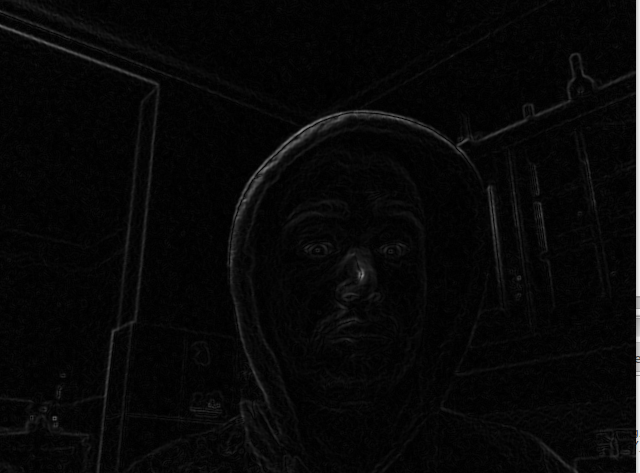
\includegraphics[width=70mm]{img/ex1.png}
\caption{Resultado obtido após exercício 1}
\end{figure}


O resultado obtido com o algoritmo de \texttt{Scharr} é o seguinte: 

%falta ver imagem esta usa os dois
\begin{figure}[ht!]
\centering
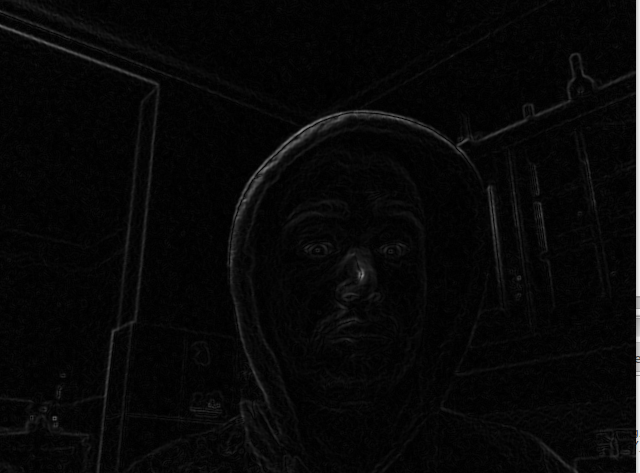
\includegraphics[width=70mm]{img/ex1.png}
\caption{Resultado obtido após exercício 1}
\end{figure}




\subsection{Problema \#2}

\subsubsection{Enunciado}
\textit{Based on the previous exercise, calculate also the Laplacian of an image. Explore the parameters
of the function and comment the results.}

\subsubsection{Resolução e principais conclusões}


Para a resolução deste exercício foram aplicadas as seguintes operações:
\begin{enumerate}
    \item Aplicação do \texttt{GaussianBlur}
    \item Conversão da imagem para grayscale através do método \texttt{cvtColor}
    \item Aplicação do método \texttt{Laplacian} 
    \item Por fim é usado o método \texttt{convertScaleAbs}
\end{enumerate}



\begin{figure}[ht!]
\centering
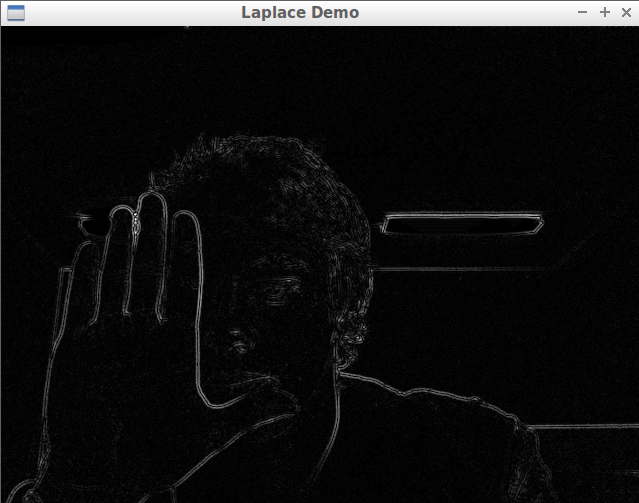
\includegraphics[width=70mm]{img/ex2.png}
\caption{Resultado obtido após exercício 2}
\end{figure}


%%%%%%%%%%%%%%%%%%%%%%%%%%%%%%%%%




\subsection{Problema \#3}

\subsubsection{Enunciado}
\textit{ Implement a program to capture images from your digital camera and perform edge detection with
Canny’s algorithm. Explore the effects of changing the parameters and comment the obtained
results.}

\subsubsection{Resolução e principais conclusões}

No problema 3 aplicámos o algoritmo de Canny diretamente e tal como nos foi dito na aula teórica, depois de ajustados os parâmetros conseguimos delinear as arestas mais importantes da imagem. Por exemplo, a imagem abaixo observámos facilmente que deteta com precisão muito mais arestas que a de cima, apenas alterando dois parametros \texttt{ratio} e o \texttt{threshold}.


\begin{figure}[ht!]
\centering
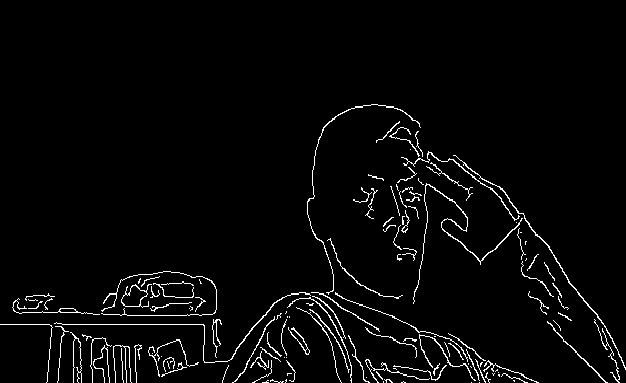
\includegraphics[width=70mm]{img/ex3.png}
\caption{Resultado após execução do problema 3.}
\end{figure}

\begin{figure}[ht!]
\centering
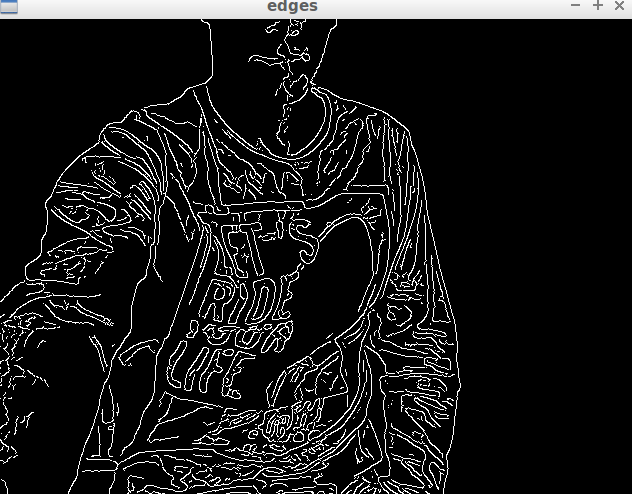
\includegraphics[width=70mm]{img/ex3better.png}
\caption{Resultado após execução do problema 3.}
\end{figure}




\newpage
%%%%%%%%%%%%%%%%%%%%%%%%
\subsection{Problema \#4}

\subsubsection{Enunciado}
\textit{Implement a program to capture images from your digital camera and perform corner detection.
Try for example the Harris’s algorithm (explore the function cornerHarris). For each corner
detected, draw a circle or a square in the image (explore the drawing functions of OpenCV).}

\subsubsection{Resolução e principais conclusões}

No problema 4 detetámos os cantos diretamente com o algoritmo de Harris abordado na aula. Pensámos não ter conseguido uma boa solução mesmo quando tentamos ajustar alguns parâmetros como o \texttt{blocksize} e o tamanho da \texttt{aperture}, mas na imagem do tutorial seguida por nós os resultados pareciam a não detetar todos os cantos também. Concluímos portanto, que a deteção de cantos é muito mais difícil que a deteção de arestas para ser executado com uma precisão elevada.

\begin{figure}[ht!]
\centering
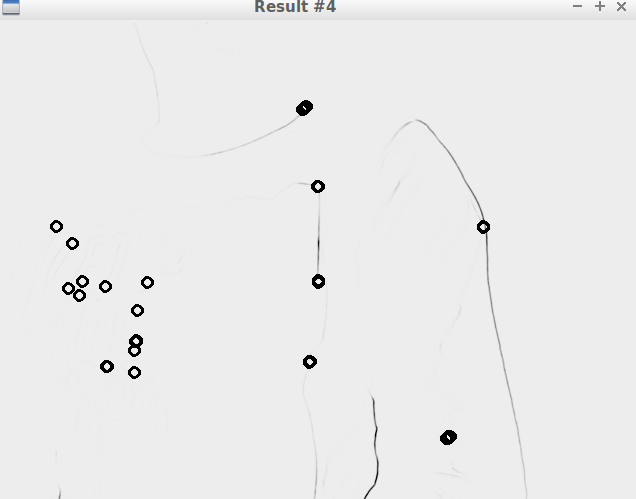
\includegraphics[width=70mm]{img/ex4.png}
\caption{Resultado após execução do problema 4}
\end{figure}

\newpage

%%%%%%%%%%%%%%%%%%%%%%%%
\subsection{Problema \#5}

\subsubsection{Enunciado}
\textit{Implement a program to detect lines and circles on an image. As suggestion, start by calculating a binary image with the edges present on the scene. Adjust the parameters to get the best edges as possible. Then explore the use of the function findContours to identify the contours
corresponding to the objects of interest.}

\subsubsection{Resolução e principais conclusões}

Este exercício irá permitir detetar todos os círculos existentes na imagem e assiná-los. Foram usados os métodos \texttt{findContours} e \texttt{approxPolyDP}. 



\begin{figure}[ht!]
\centering
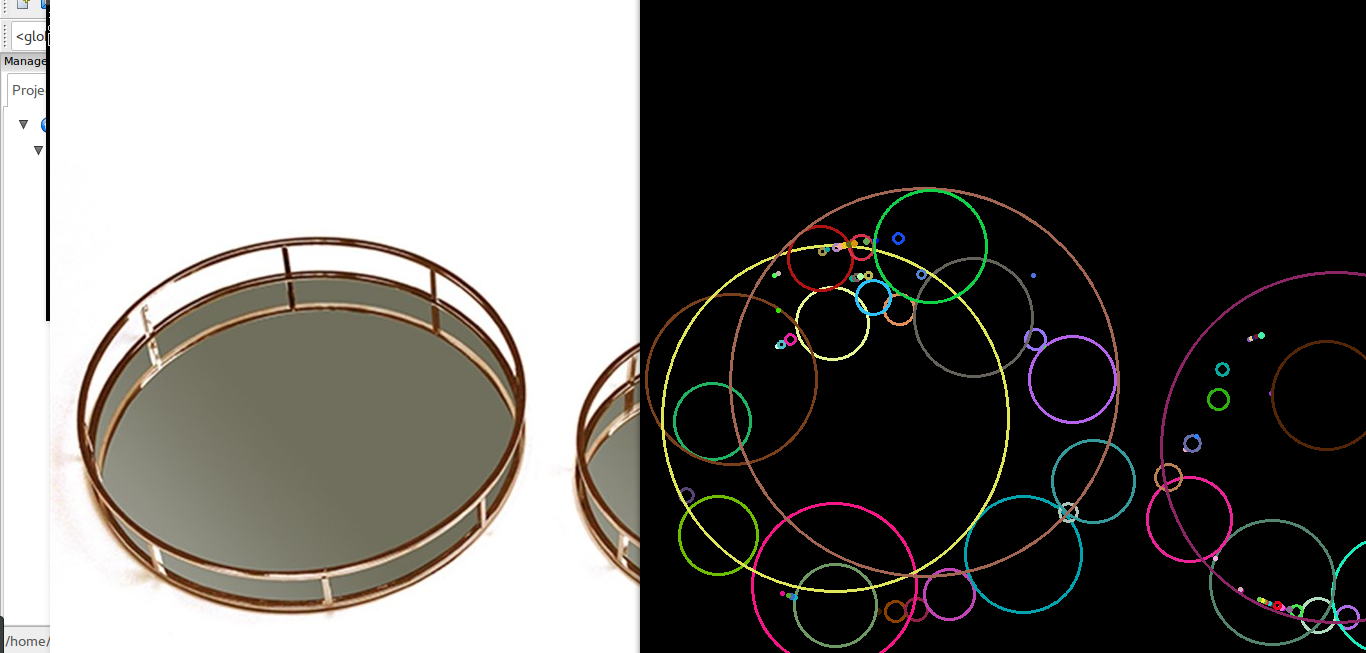
\includegraphics[width=70mm]{img/ex5.png}
\caption{Resultado após execução do problema 5 }
\end{figure}

\subsection{Problema \#6}

\subsubsection{Enunciado}
\textit{Implement a different solution for the previous problem using the Hough Line Transform and the Hough Circle Transform.}

\subsubsection{Resolução e principais conclusões}

Para a resolução deste exercício foram realizados dois tutoriais do OpenCV: 

\begin{itemize}
    \item \textit{Hough Line Transform}\\
    Foram executadas as seguintes operações: 
    \begin{enumerate}
        \item Foi aplicado o método \texttt{Canny} ao imagem inicial, neste caso imagem proveniente da câmara. 
        \item Foi usado o \texttt{cvtColor} para obter um conversão para \texttt{CV\_GRAY2BGR}
        \item Foi usado o método \texttt{HoughLinesP}
        \item E por fim, o método \texttt{line}
    \end{enumerate}
    
\begin{figure}[ht!]
\centering
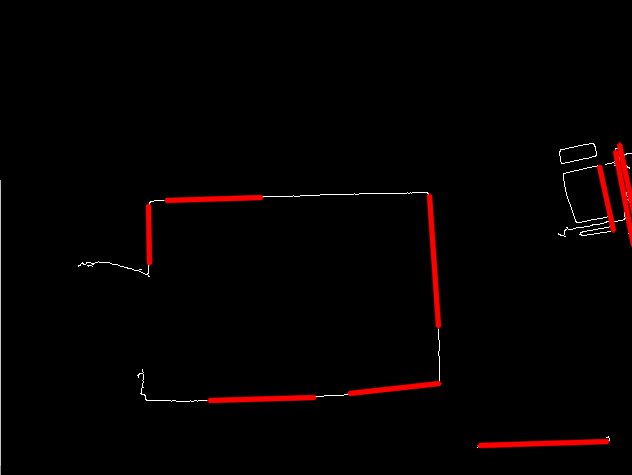
\includegraphics[width=70mm]{img/ex6_1.png}
\caption{Resultado após execução do \textit{Hough Line Transform}}
\end{figure}

    \newpage
    
    \item \textit{Hough Circle Transform}
    Foram executadas as seguintes operações: 
    \begin{enumerate}
        \item Foi usado o \texttt{cvtColor} para obter um conversão para \texttt{CV\_GRAY2BGR}
        \item Para reduzir o ruído foi usado o método \texttt{GaussianBlur}
        \item Foi usado o seguinte método \texttt{HoughCircles} para encontrar todos os círculos presentes na imagem
        \item Por fim, foi usado o método \texttt{circle} para desenhar o circulo detectado. 
    \end{enumerate}

\begin{figure}[ht!]
\centering
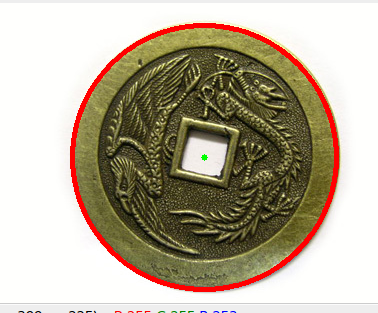
\includegraphics[width=70mm]{img/ex6_2.png}
\caption{Resultado após execução do \textit{Hough Circle Transform}}
\end{figure}

\end{itemize}





\begin{thebibliography}{1} % 9



\bibitem{fsound}
Neves, A. J. R.; Dias, P. Slides teóricos Visão por Computador - Aula 4 (2016)


\bibitem{vtk}
OpenCV. \href{hhttp://docs.opencv.org/}{Opencv Documentation}. Web. 15 Outubro 2016. 




\end{thebibliography}

\end{document}
